\section{Experiment}
\label{ch4-sec:experiment}

In this section, we first describe the datasets and experimental settings. Then we quantitatively evaluate our method on two separate prediction tasks. Finally, we present two case studies to intuitively explain the strength of our methods. 


\subsection{Experiment Setting}  \label{data:sets}

\subsubsection{Data description}
The fundamental geographic unit of study in this paper is a tract, which is a small area established by the U.S. Census Bureau for analyzing populations. We use the tract as the unit of study, because it offers the finest granularity for which demographic data is recorded. The following data are used in this paper, and a summary of the data property is given in Table~\ref{tab:data-summary}.

\begin{table}
\centering
\caption{Data set property}
\label{tab:data-summary}
\begin{tabular}{|l|l|r|r|l|}
\hline
Data set & Granularity & \#Sample & \#Field & Year \\ \hline
Demographics & tract & 801 & 110 & 2010 \\ \hline
Map & tract & 801 & - & 2010 \\ \hline
Crime & point-wise & $719,461$ & 16 & 2010-2011 \\ \hline
House price & point-wise & $44,447$ & 14 & 2015-2017 \\ \hline
\end{tabular}
\end{table}

\textbf{Demographic Data}. Socioeconomic and demographic features of neighborhoods have been widely used to predict crime \cite{wang2016simple}. We collect the demographic data of 801 tracts in Chicago from 2010 US census survey~\cite{census:2010}. The demographics data provide the raw count of households over 100 different categories, include ethnicity, income, education, etc.

\textbf{Map Data}. The geographic boundary information for 801 tracts are available through the U.S. census survey~\cite{census:2010} as well. Each boundary is defined by a polygon with a sequence of GPS coordinates.

\textbf{Crime Data}. The Chicago Data Portal~\cite{data-crime} provides the detailed records of over five million incidents of crime from 2011 - 2017. Our study focuses on year 2010 and 2011 only. For each crime incident, the date, location, and incident type are reported. 

\textbf{House Price Data.} House price data in the Chicago metropolitan area are obtained from Zillow, a popular real estate website~\cite{data-houseprice}. We collect the last sale price, floor size, latitude,  and longitude information for over $44,000$ properties that were sold between January 2015 and December 2017.


\subsubsection{Prediction Tasks}


We employ a negative binomial regression model~\cite{wang2016crime} as our prediction task, namely
\begin{equation*}
\mathbf{E}(Y) = \exp( \alpha X ),
\end{equation*}
where $\mathbf{E}$ calculates the expectation. The link function used in the regression is a negative binomial distribution. The advantages of negative binomial regression are two-fold. First, a negative binomial model is suitable for non-negative value prediction. Second, compared to Poisson regression, negative binomial regression solves the over-dispersion problem by allowing the variance to be larger than the mean.

The demographics features at the community level are used as contextual features $X_i$. Note that it is not feasible to directly use the raw count in the demographic data as $X$. We pre-process the raw counts into mutually independent features, such as total population, percentage of household in each income category, diversity of ethnicity, etc.


Two prediction tasks are used to evaluate our region partition methods in the experiments. Both tasks use the same processed demographic features as $X$. The first task is crime count prediction, where we aggregate the total number of crime in a community as $Y$. The crime count in year 2010 is used as training data, and the crime count in 2011 is used as testing data. The second task is house price prediction, where we use the average price per square foot in a community as $Y$. The houses that are sold before August 1st, 2016 are used as training data, while the rest are used as testing. The split point makes the training and testing data have a roughly equal number of samples.




\subsubsection{Compared Methods}

The existing administrative boundary is a clear baseline partition. Since our region partition problem is similar to clustering problem, we employ various conventional clustering methods to derive different clustering partitions as alternative baselines. More specifically, we compare the following region partition methods.



\begin{figure*}[t!]
\centering
\subfigure[\texttt{Agglomerative}]{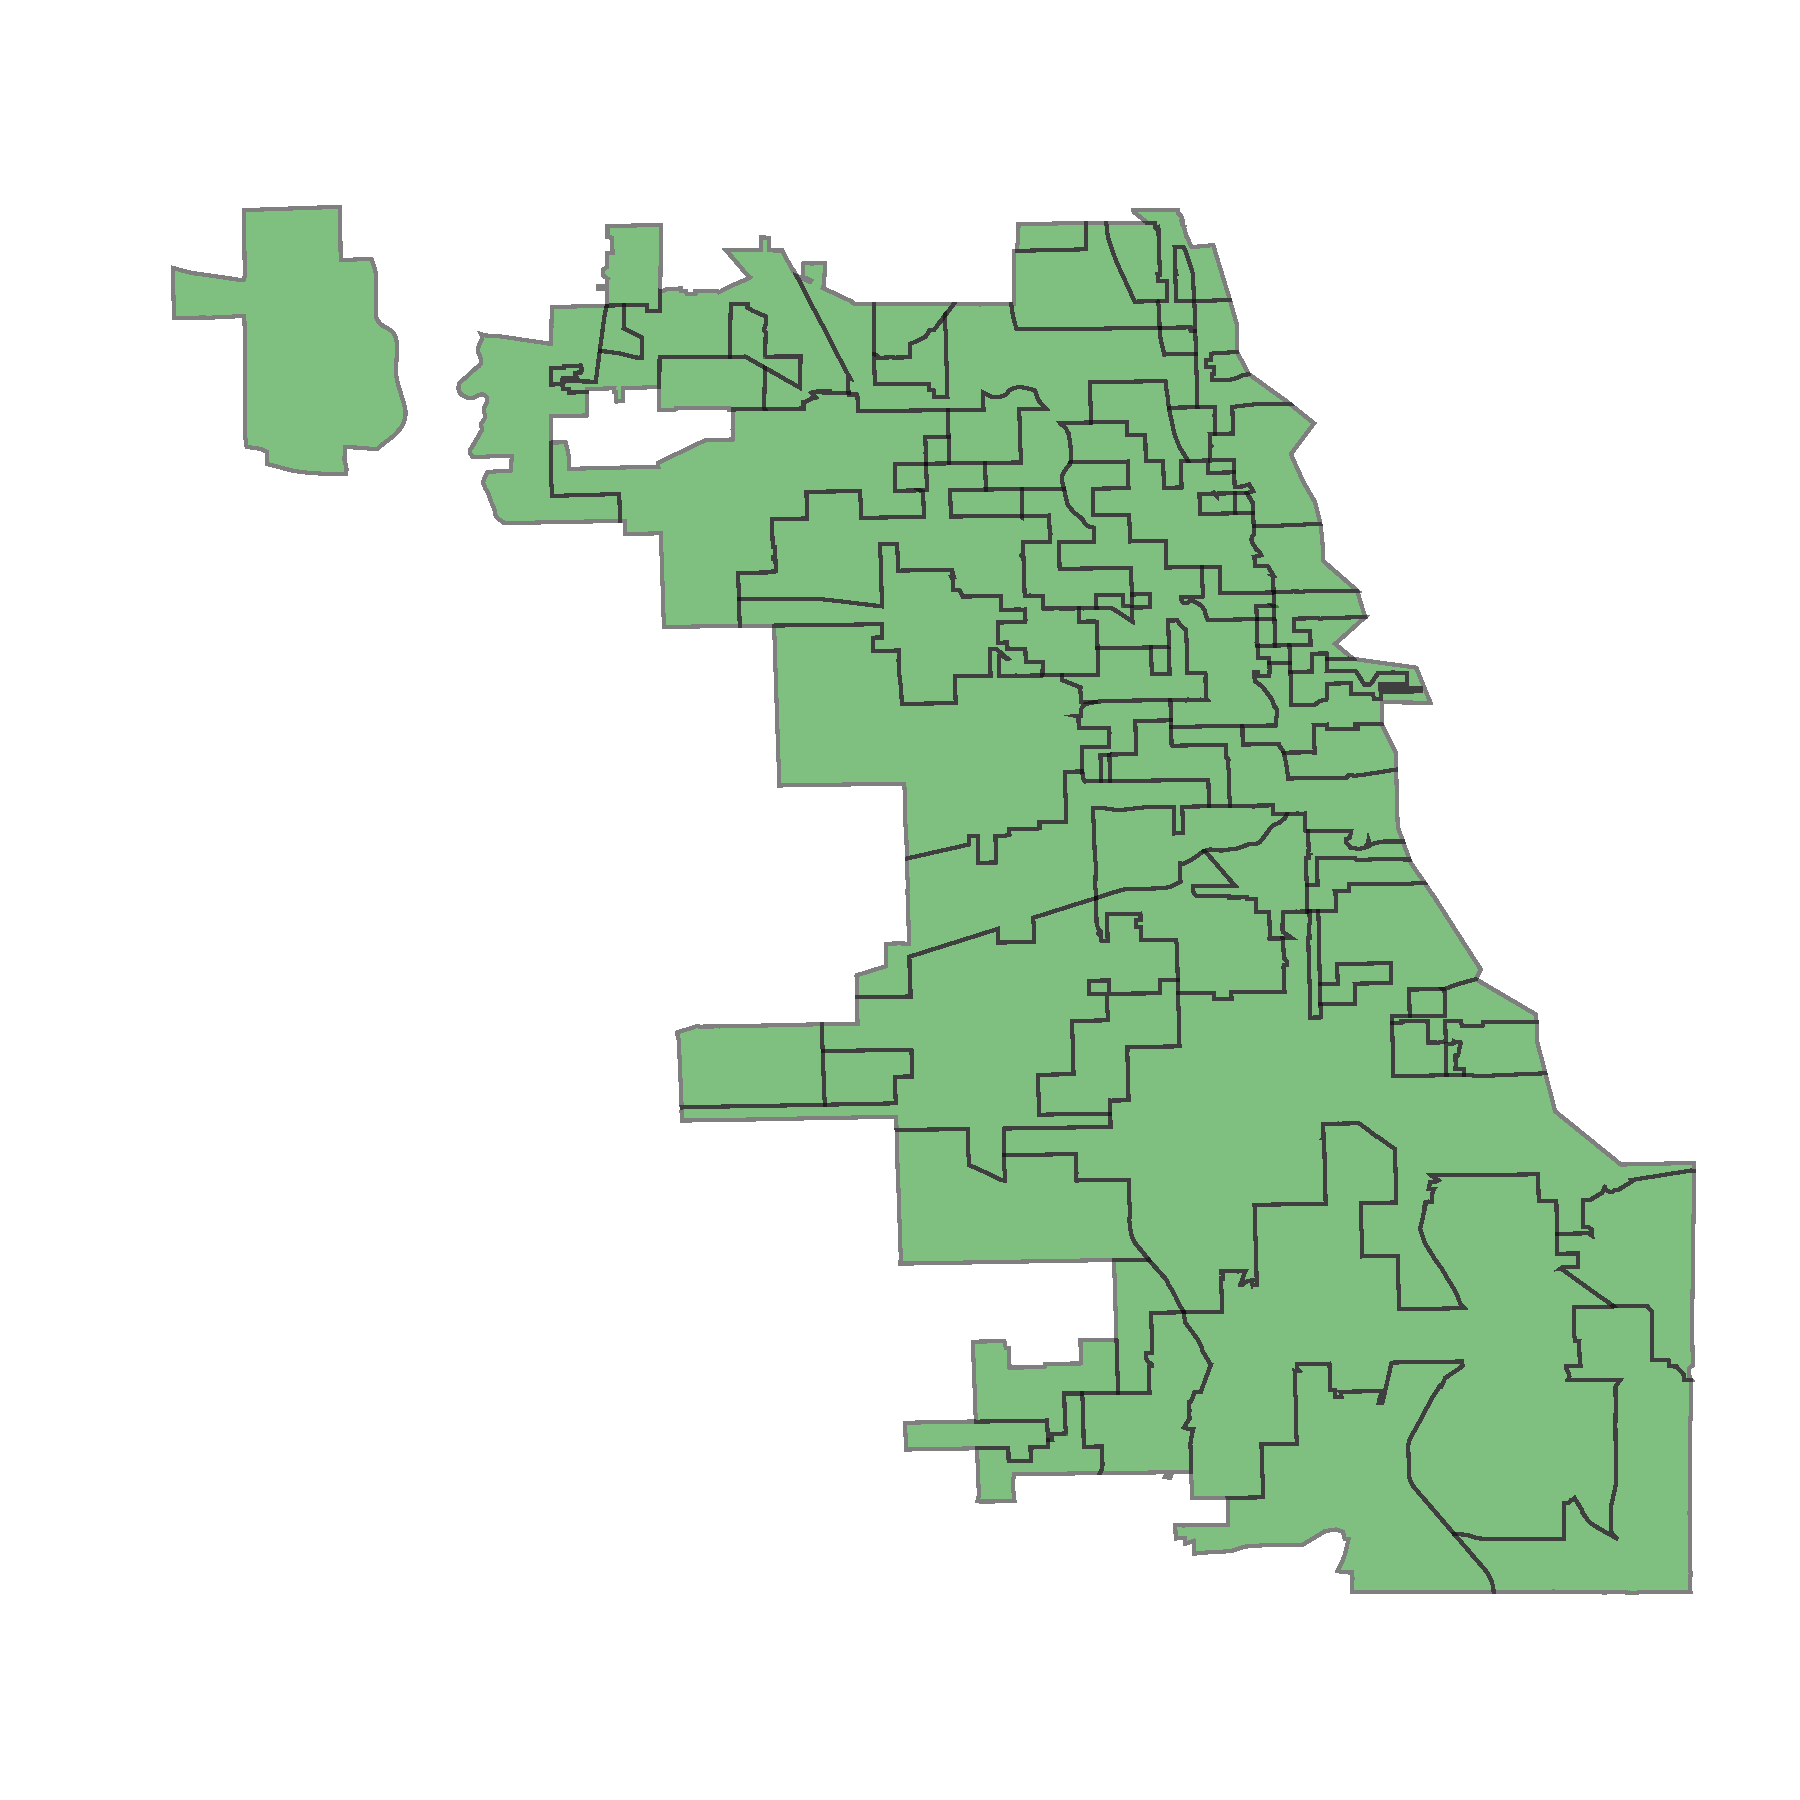
\includegraphics[width=0.45\linewidth]{fig/agg_CAs.pdf}}
\subfigure[\texttt{K-Means}]{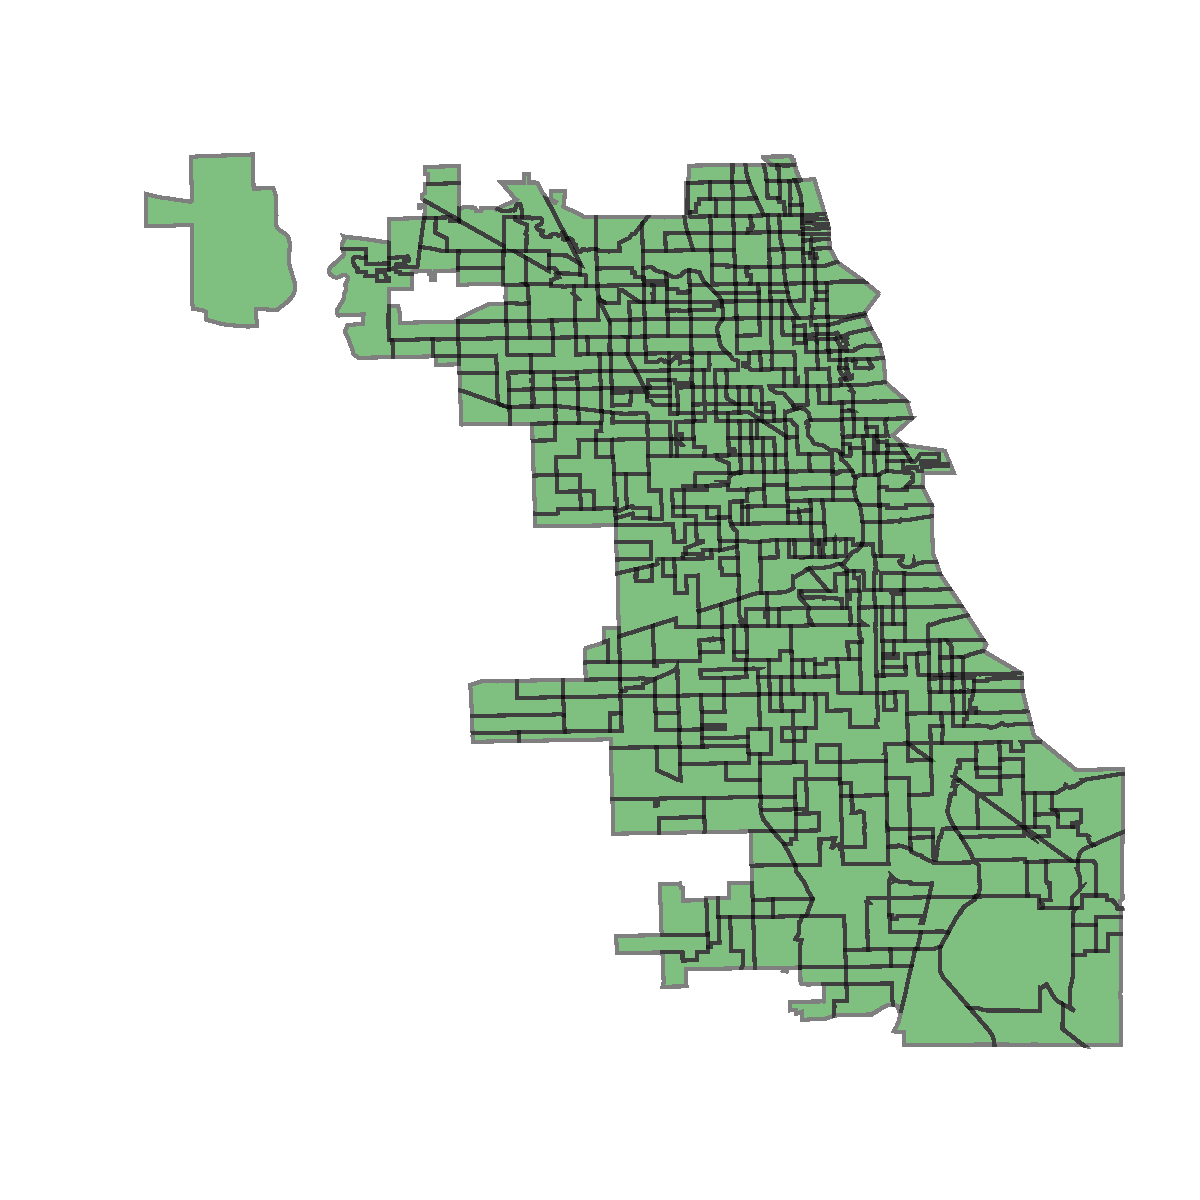
\includegraphics[width=0.45\linewidth]{fig/kmeans_CAs.pdf}}
\subfigure[\texttt{Spectral}]{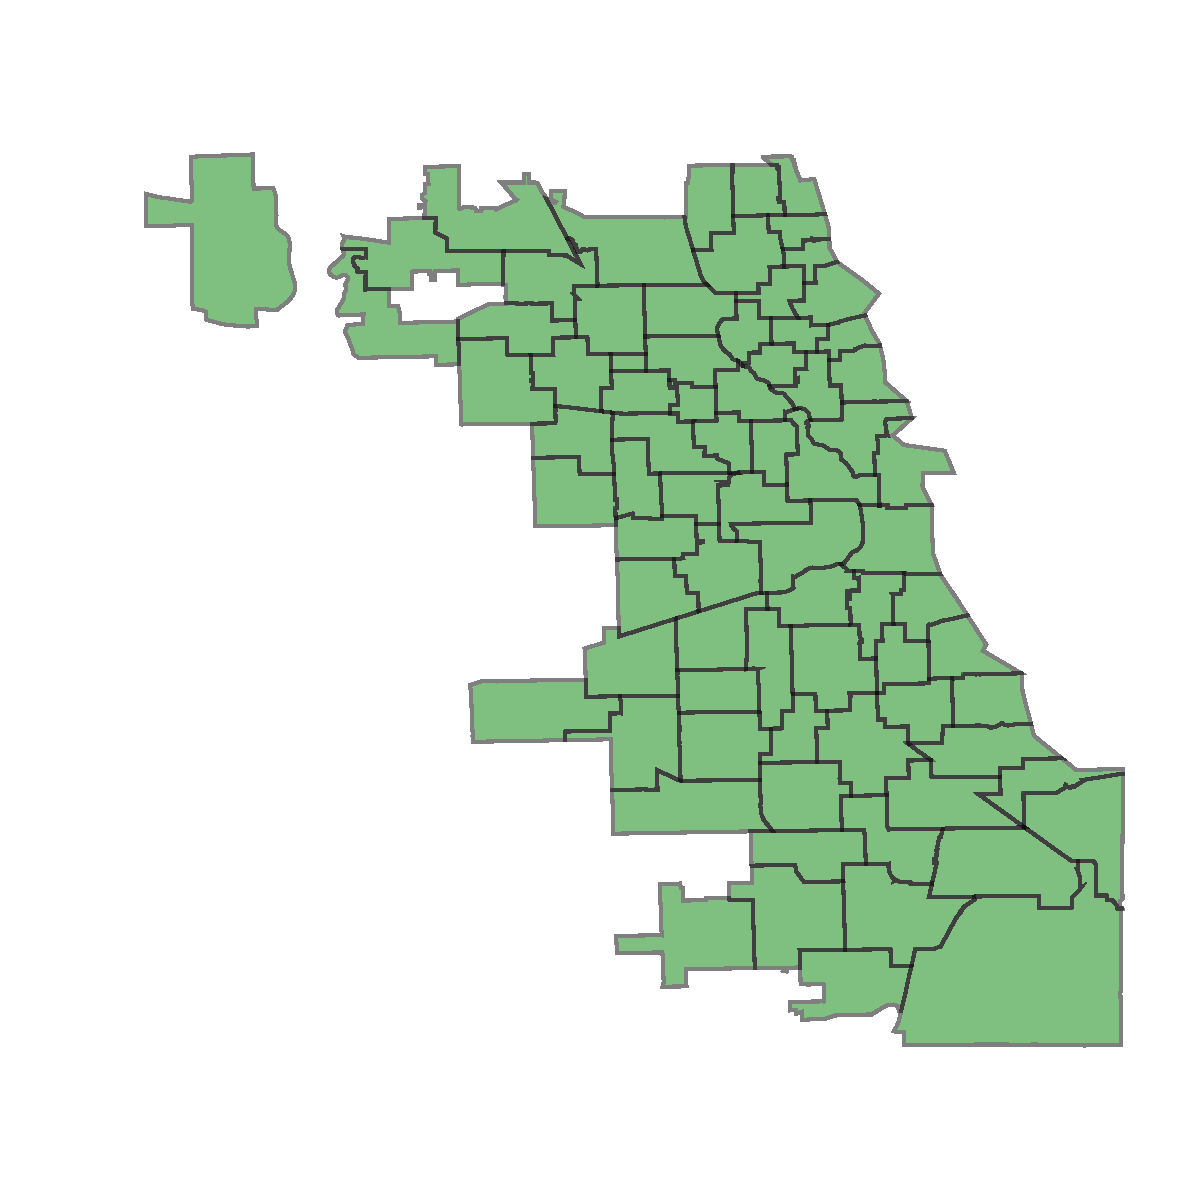
\includegraphics[width=0.45\linewidth]{fig/spectral_CAs.pdf}}
\subfigure[\texttt{DQN}]{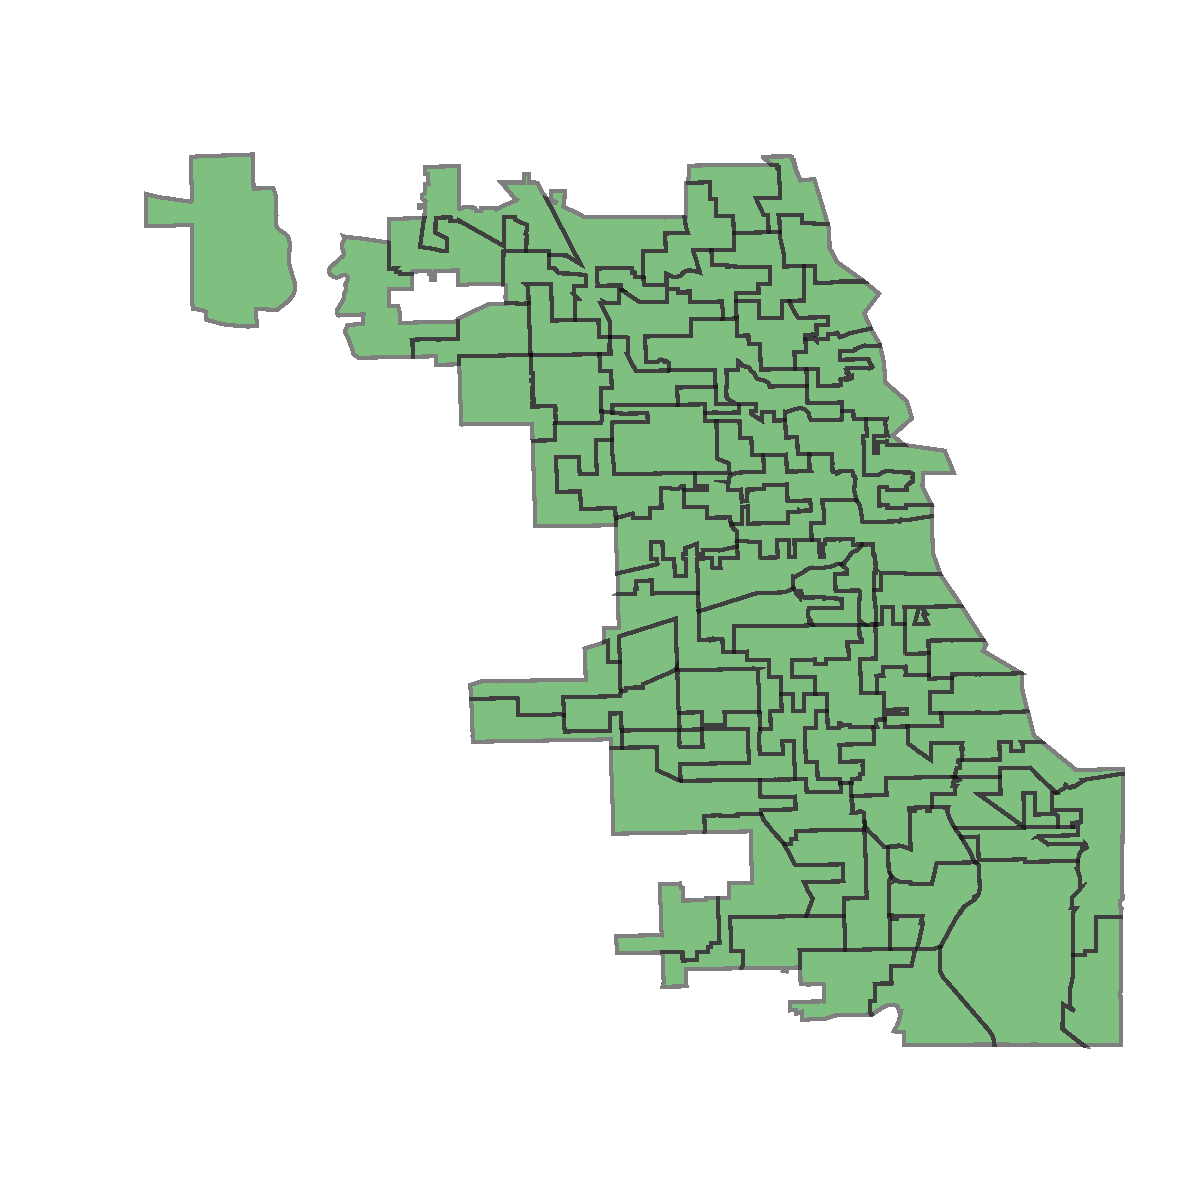
\includegraphics[width=0.45\linewidth]{fig/case-study-house-price-q-learning-v10-CAs.pdf}}
\caption{(a - c) The clustering results for three clustering baselines. (d) The learned partition from \texttt{DQN} method for crime prediction task.}
\label{fig:partitions}
\end{figure*}



\begin{itemize}[leftmargin=*]
\item \textbf{(\texttt{Admin})} Administrative boundary  uses the existing administrative boundary defined by US Bureau of Census~\cite{census:2010}. A visual depiction of this partition can be seen in Figure~\ref{fig:intro}. %This baseline partition is denoted as \texttt{Admin}. 
\item \textbf{(\texttt{Agglomerative})} Agglomerative clustering performs a hierarchical clustering using a bottom up approach. The ward linkage function is used, along with a tract adjacency graph as input to guarantee spatial continuity. %This method is denoted as \texttt{Agglomerative}.
\item \textbf{(\texttt{K-Means})} K-means clustering separates tracts into $n$ groups of equal variance.%, denoted as \texttt{K-Means}.
\item \textbf{ (\texttt{Spectral})} Spectral clustering does a low-dimensional embedding of the affinity matrix between samples first, and then applies the K-means method in the lower dimensional space. Note that \texttt{Spectral} also takes the tract adjacency graph as the affinity graph.
\item \textbf{(\texttt{Naive})} MCMC with naive proposal. The first variant of our proposed MCMC method using a straightforward uniform proposal.
\item \textbf{(\texttt{Softmax})} MCMC with softmax proposal is another variant of our MCMC method, which uses strong heuristics.
\item \textbf{(\texttt{DQN})} Q-learning is our proposed reinforcement learning method to search for optimal partition.
\end{itemize}

For various clustering methods, we set the number of clusters as $m=77$, which equals the number of community areas in \texttt{Admin}. Note that if we run clustering methods multiple times, they usually produce the exact same clustering results. The MCMC and \texttt{DQN} methods, on the other hand, are all stochastic processes and do not converge to the same partition. Therefore, we run $100$ rounds of our proposed methods and report the average measure.



\subsubsection{Evaluation Metrics} 


Given a partition $\mathcal{Z}$, we evaluate the quality of this partition on the testing data set.
Mean absolute error (MAE) is used to measure the performance of prediction tasks, i.e.
\begin{equation}
MAE = \frac{ \sum_{j=1}^m |Y_j - \hat{Y_j}| }{ m},
\end{equation}
where $\hat{Y_i}$ is the leave-one-out prediction error of community $Z_j$. Namely, we train a model on the rest of the communities $\mathcal{Z} \setminus Z_j$. Then, $\hat{Y_j}$ is the estimated target value for $Z_j$ from the trained model.


\subsection{Quantitative Evaluations}

\subsubsection{Effectiveness Study}

In Table~\ref{tab:mae}, we report the evaluation results of the various partition methods. The partitions results from different baselines are visualized in Figure~\ref{fig:partitions}(a-c). Since our methods are run for 100 rounds, we report both the MAE and its standard deviation in the table. The final partition of \texttt{DQN} is visualized in Figure~\ref{fig:partitions}(d). Overall, we have the following three observations.


\begin{table}[h!]
\centering
\caption{Prediction MAEs of various partition methods. Our proposed methods are run for 100 rounds. The MAE and its variance are reported.}
\label{tab:mae}
\begin{tabular}{ |c|>{\raggedleft\arraybackslash}p{4cm}|>{\raggedleft\arraybackslash}p{4cm}|} 
\hline
 Method & \multicolumn{2}{c|}{MAE}  \\ \hline
   & Crime & House price \\
 \hline
 \texttt{Admin} & 1715.91 & 31.29  \\ 
 \hline
 \texttt{Agglomerative} & 72201.00 & 50.34 \\
 \hline
 \texttt{K-means} & 2887.83 & 32.40 \\
 \hline
 \texttt{Spectral} & 1440.57 & 29.66  \\
 \hline
 \texttt{Naive} & 1073.42(81.93) & 25.73(2.76) \\
 \hline
 \texttt{Softmax} & 1041.68(76.75) & 27.13(2.98) \\
 \hline
 \texttt{DQN} & \textbf{746.13}(154.19) & \textbf{25.16}(1.30) \\
 \hline
\end{tabular}
\end{table}


\emph{Clustering methods overall perform poorly}. This is likely due to the fact that the clustering methods do not consider the task information. More specifically, \texttt{Agglomerative} results in the highest prediction errors for both crime prediction and house price prediction task. The reason is that  \texttt{Agglomerative} method utilizes tract connectivity as a hard constraint. As a result, the generated communities have a large variance in their sizes, as shown in Figure~\ref{fig:partitions}(a).  \texttt{K-Means} gives worse result than that of \texttt{Admin} as well. The generated partition of \texttt{K-Means} seems to consist of more than $m$ communities in Figure~\ref{fig:partitions}(b) because \texttt{K-Means} does not incorporate spatial continuity constraint. Consequently, one community can consist of several disconnected components.  \texttt{Spectral} methods generates the best results in both tasks among these baselines because \texttt{Spectral} accounts for the affinity of tracts and generates communities with similar sizes. However, it is worth mentioning that  \texttt{Spectral} method cannot guarantee the spatial continuity of generated communities. From Figure~\ref{fig:partitions}(c), we can also see that \texttt{Spectral} shows similar partition as the original administrative boundary, shown in Figure~\ref{fig:intro}(a). That is also why it achieves similar prediction accuracy as \texttt{Admin}.



\emph{The proposed MCMC method outperforms the baselines}. Both variants of MCMC methods significantly outperform  \texttt{Admin} and \texttt{Spectral} baselines. Such observations validate the effectiveness of the MCMC strategy in searching for optimal solutions. However, it is not conclusive to say \texttt{Softmax} is better than \texttt{Naive}, because while \texttt{Softmax} has better performance on crime prediction task,  \texttt{Naive} has better performance in house price prediction. The reason could be that the heuristics used in \texttt{Softmax} is not universally applicable. The heuristic assumes that working on a community with the highest error will lead to optimal solution. When this heuristic is wrong, it aggressively reduces the search space, excluding where there are better local optimal partitions. 



\emph{ \texttt{DQN} method performs the best among all}. It is clear that  \texttt{DQN} finds a better local optimal solution than that of MCMC methods. On the crime prediction task, the average MAE is $746.13$, which represents a $56\%$ improvement over  \texttt{Admin} baseline. On the house price prediction task, \texttt{DQN} consistently gives the best performance. The reason is that \texttt{DQN} explores over a subset of actions and picks the best one at each step, compared to the MCMC method, which searches the partition space in a depth first search fashion. Comparing the final partition of \texttt{DQN} and \texttt{Spectral}, we will notice that \texttt{Spectral} partition is more similar to the original administrative boundary in Figure~\ref{fig:intro}. As a consequence,  \texttt{Spectral} has similar MAE to \texttt{Admin}, but is much worse than \texttt{DQN}.


\begin{figure}[t!]
\centering
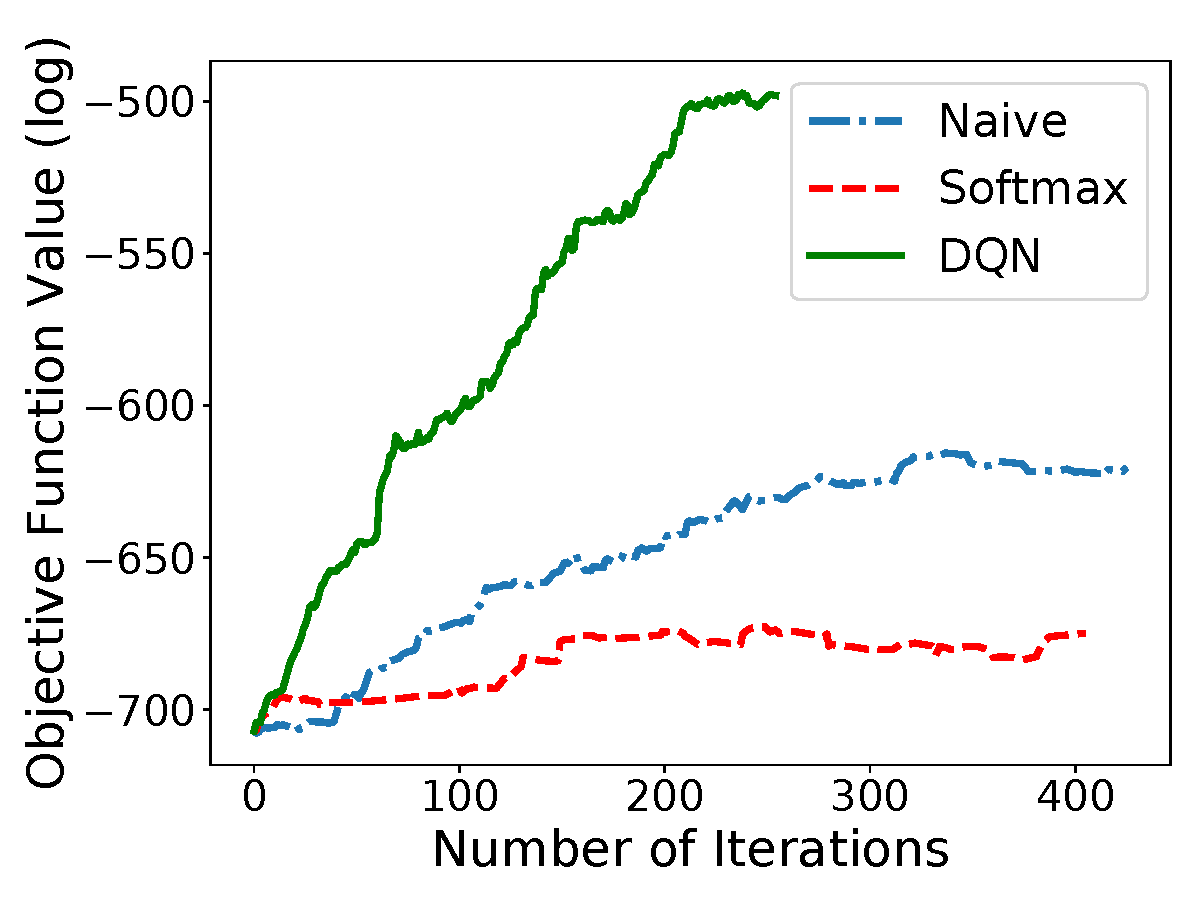
\includegraphics[width=0.9\linewidth]{fig/convergence-study.pdf}
\caption{Convergence plots for proposed methods on house price prediction task.}
\label{fig:convergence}
\end{figure}



\begin{figure*}[t!]
\centering
\subfigure[All communities]{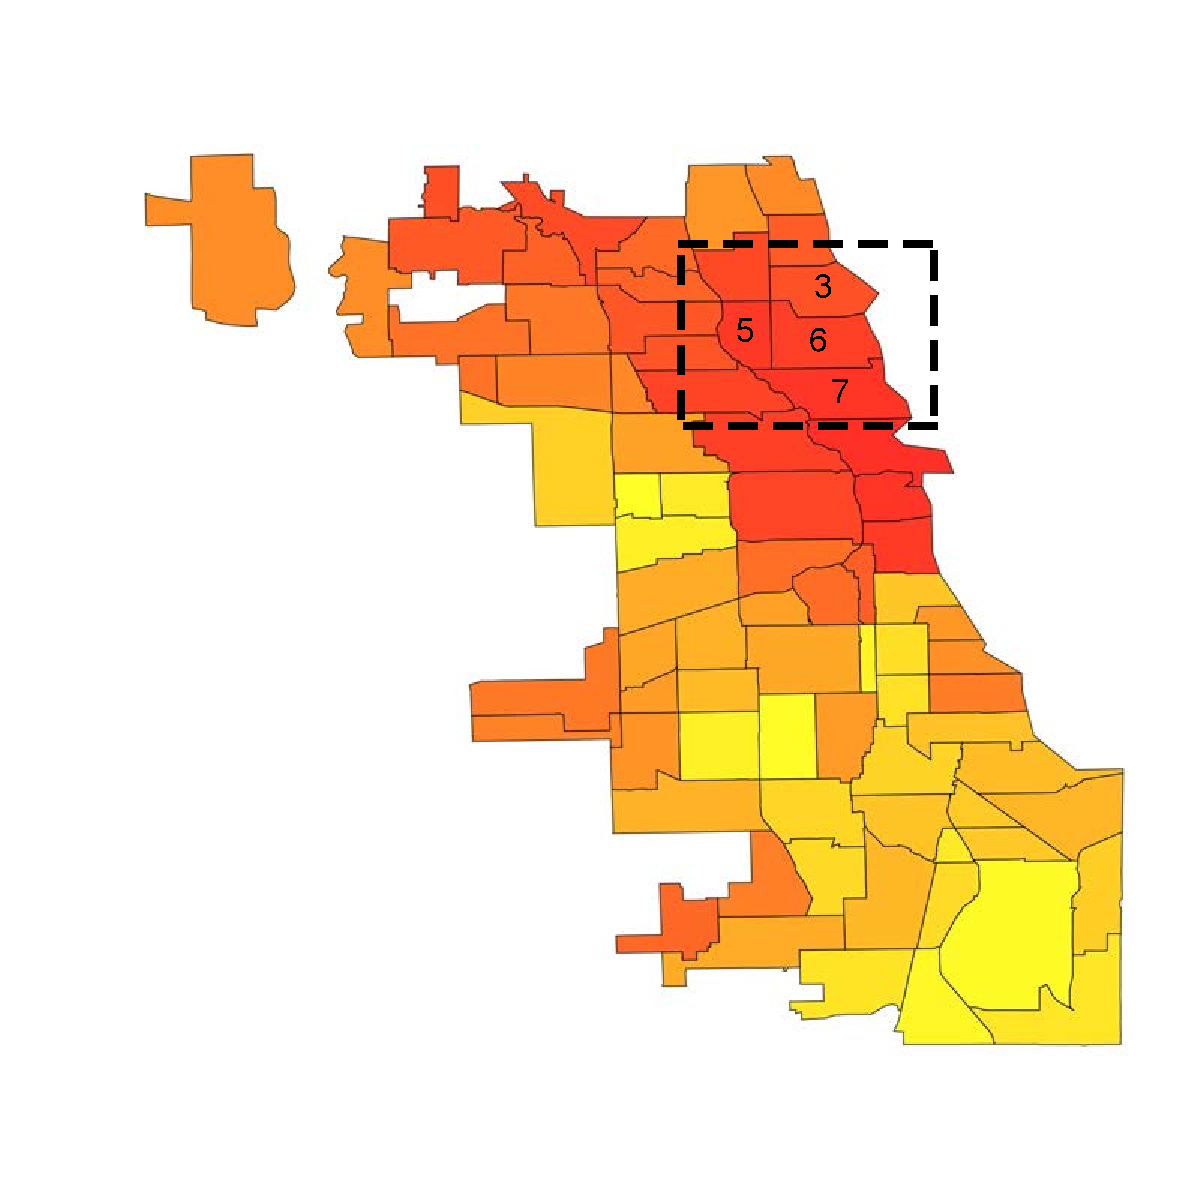
\includegraphics[width=0.3\linewidth]{fig/before-train_average_house_price-all-final.pdf}}
\subfigure[Before]{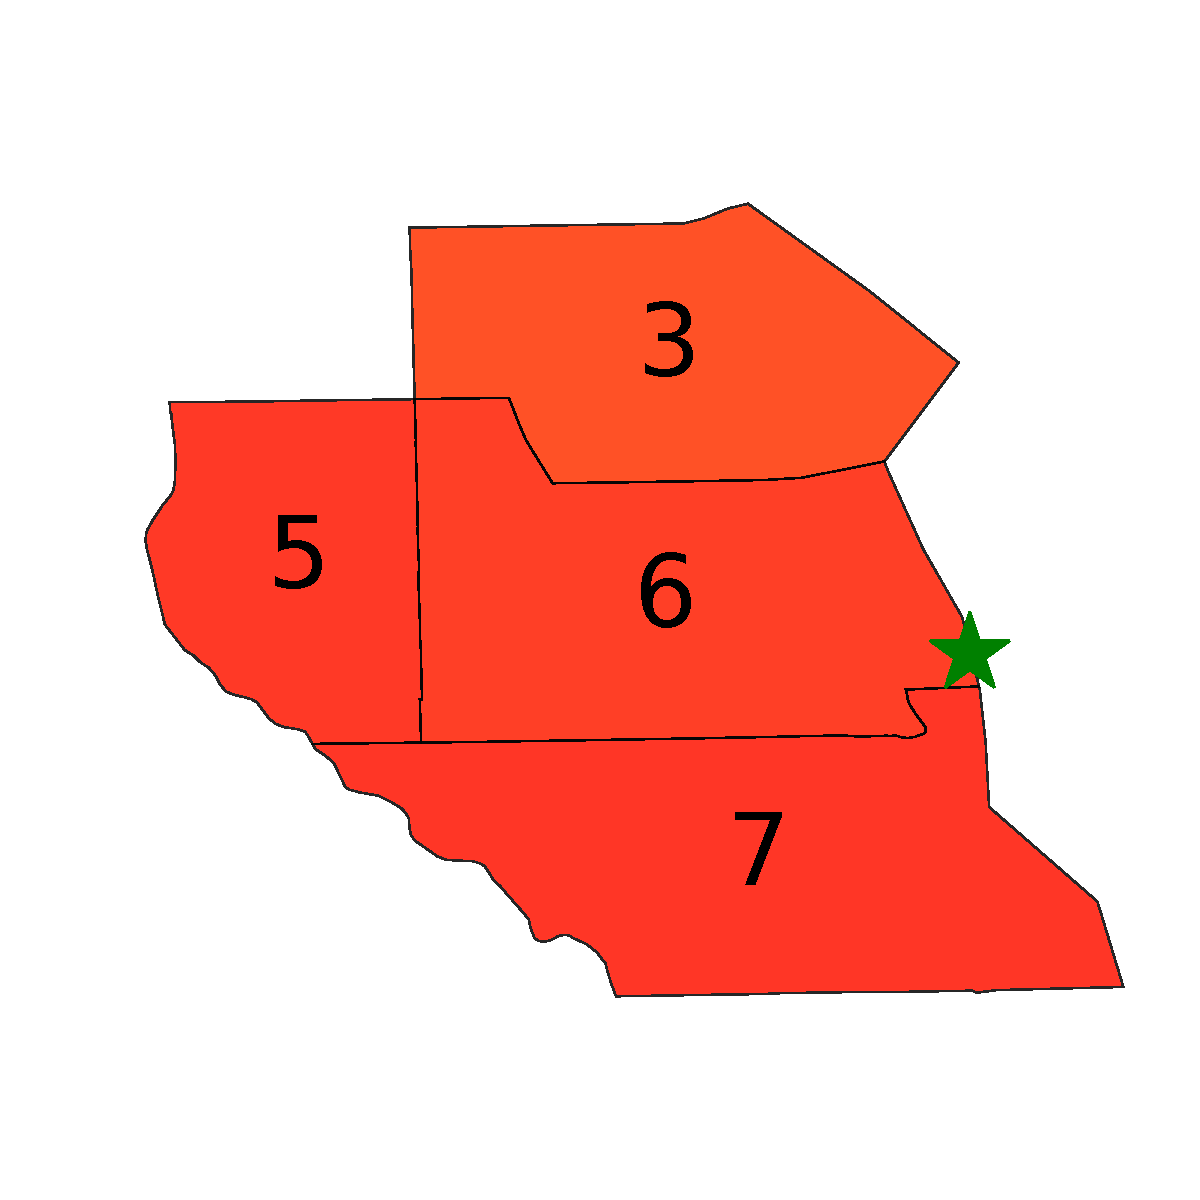
\includegraphics[width=0.28\linewidth]{fig/before-train_average_house_price.pdf}}
\subfigure[After]{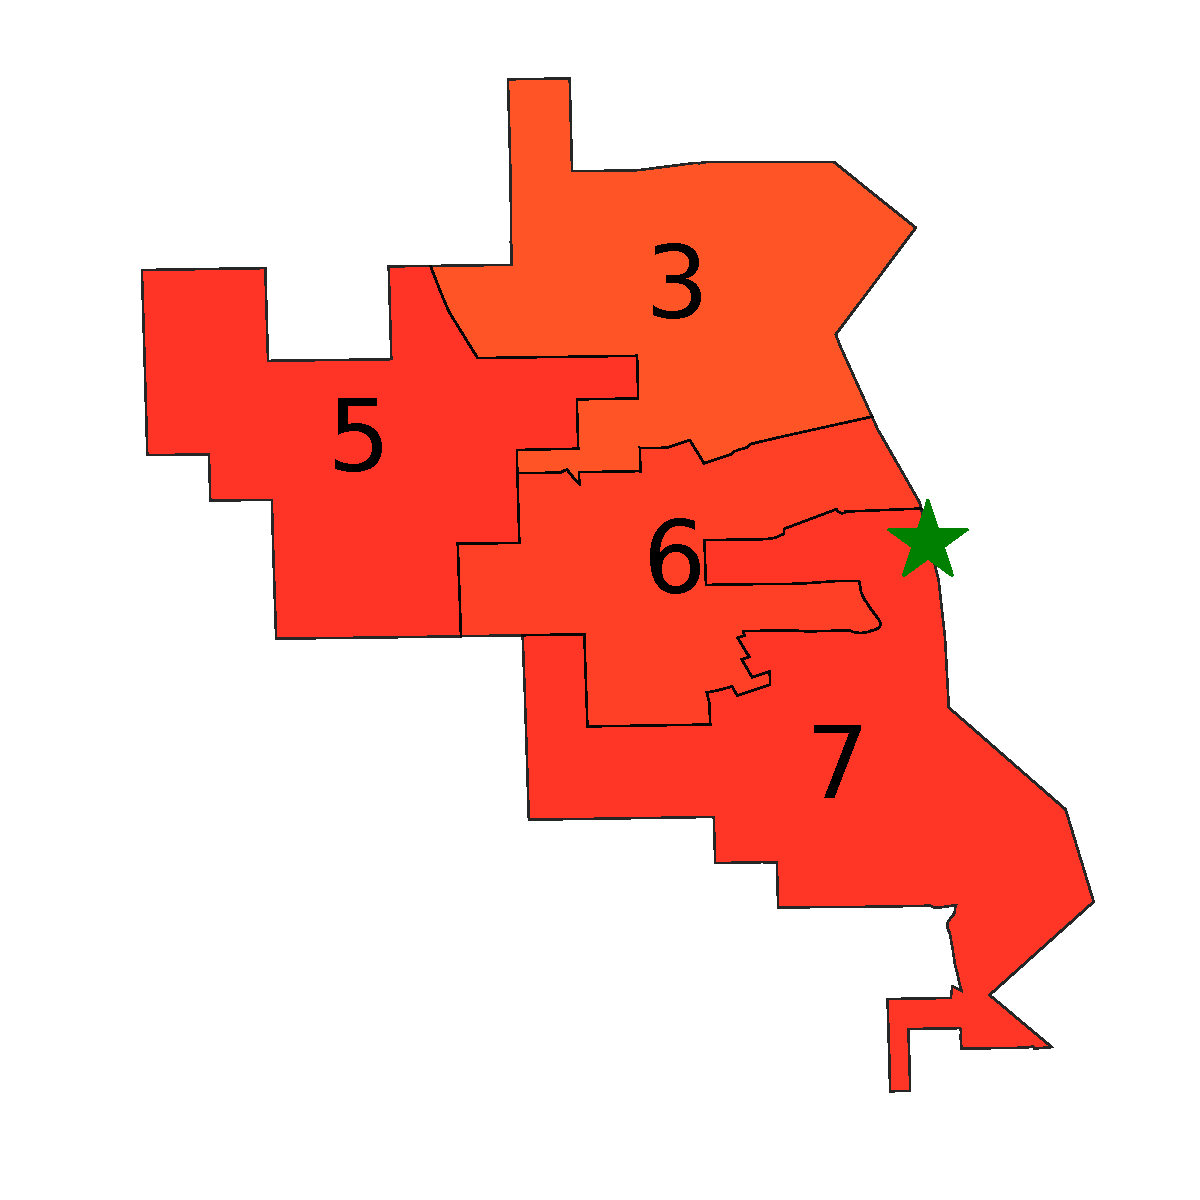
\includegraphics[width=0.3\linewidth]{fig/after-train_average_house_price.pdf}}
\subfigure[Lake View]{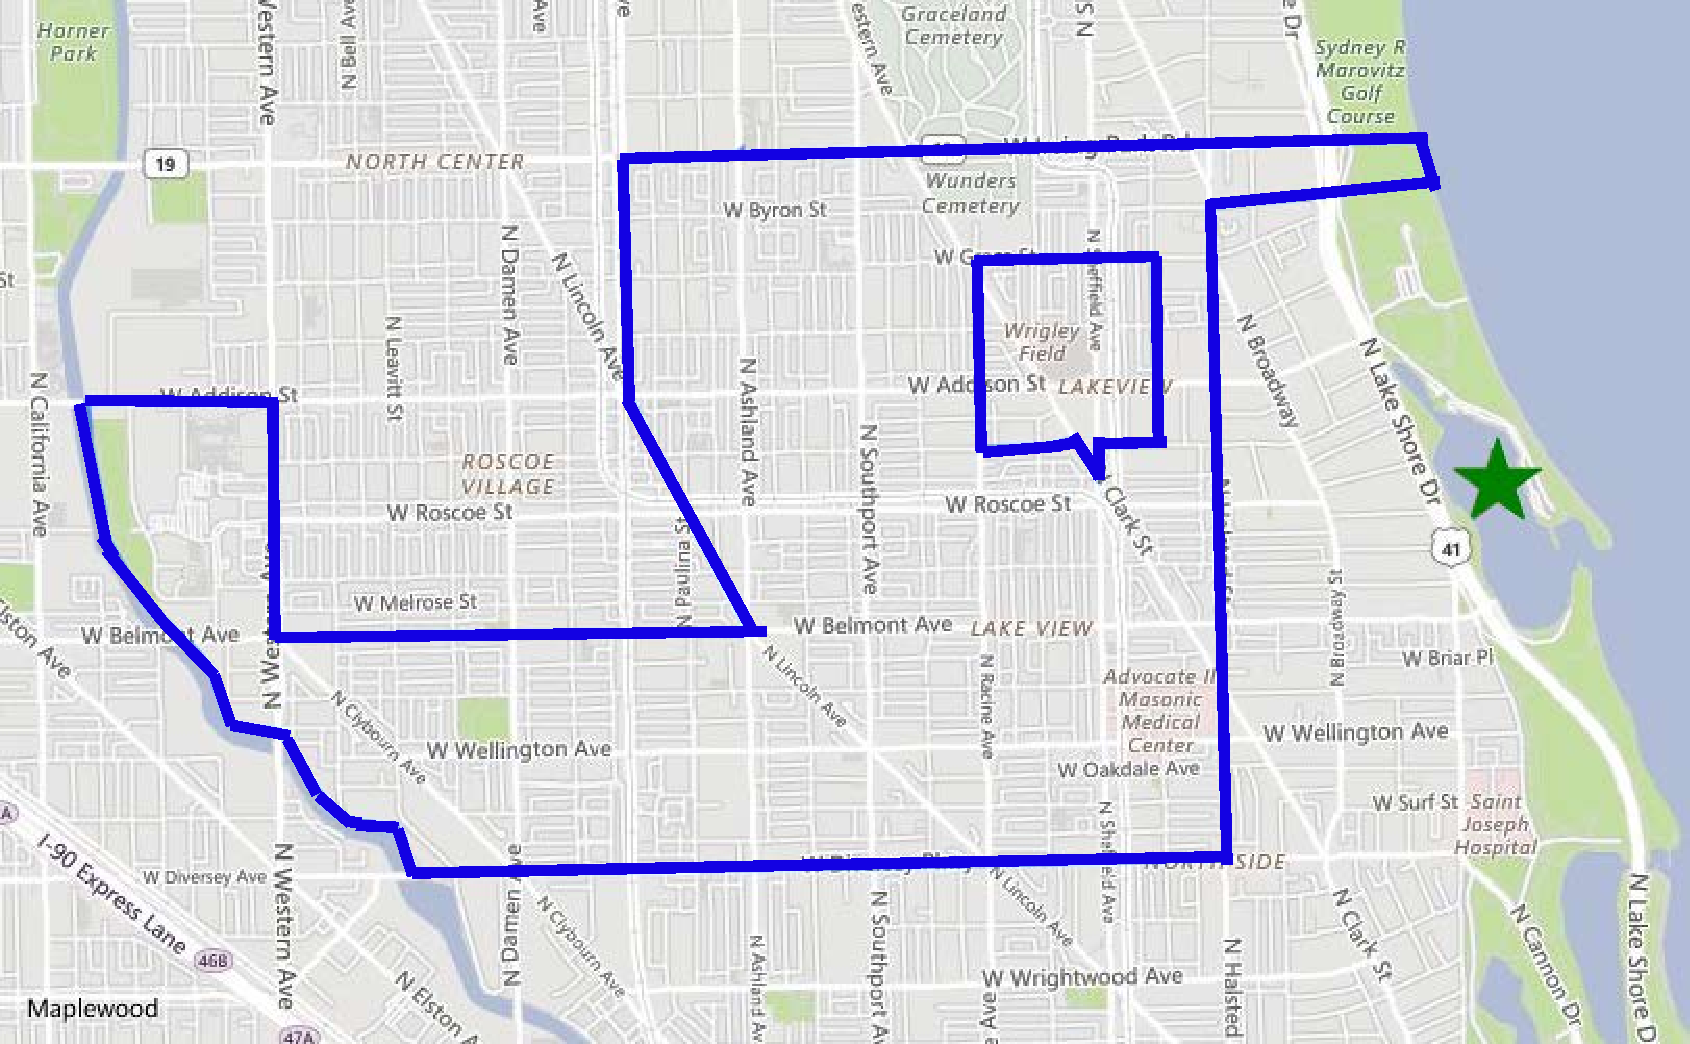
\includegraphics[width=0.45\linewidth]{fig/ca-lakeview.pdf}}
\subfigure[Lake View East]{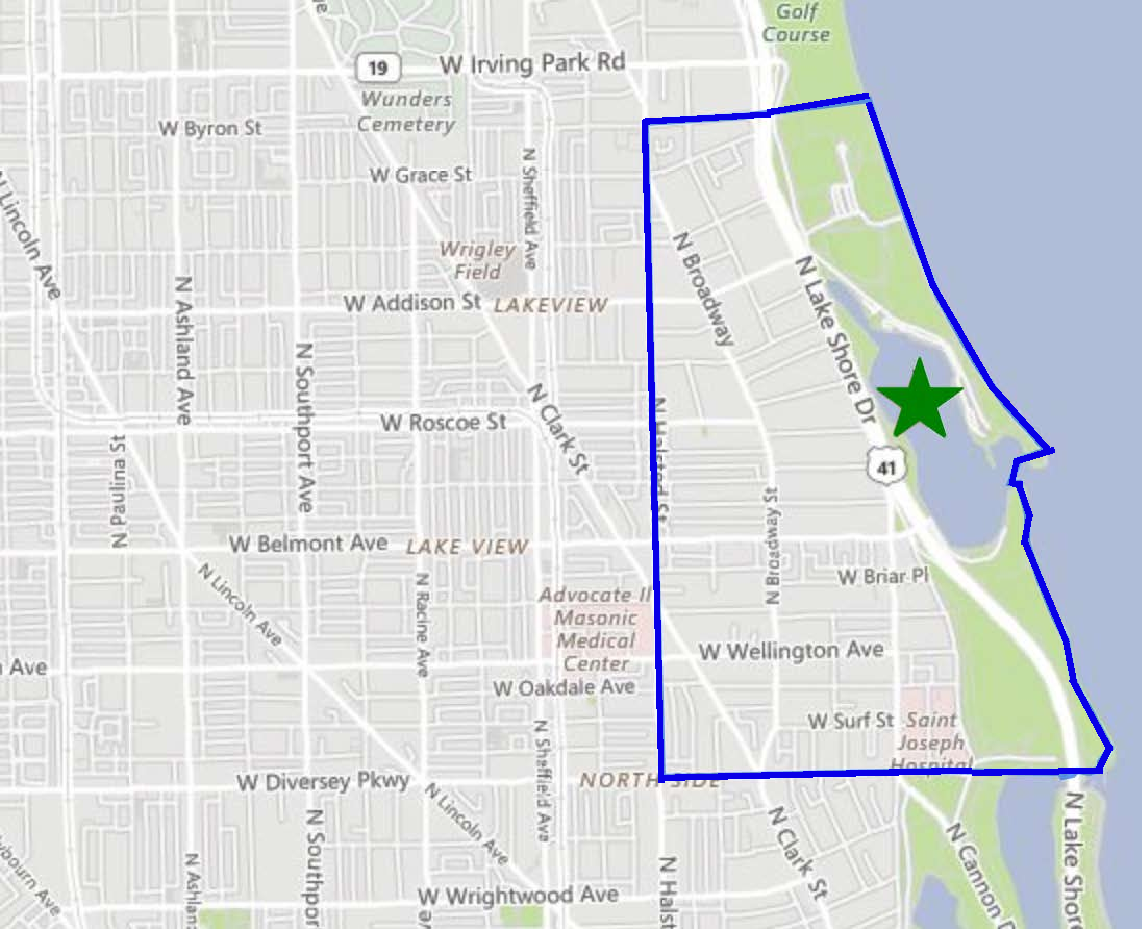
\includegraphics[width=0.34\linewidth]{fig/ca-lakeview-east.pdf}}
\caption{House price prediction case near Belmont Harbor, denoted by green star. (a) Average house price distribution in Chicago under \texttt{Admin} partition. Dotted rectangle denotes region of interest. (b) Region of interest under \texttt{Admin} partition. (c) Region of interest under \texttt{DQN} partition. (d - e) Region of interest according to Zillow. Note that the Belmont Harbor area is split into a separate community, named Lake View East.}
\label{fig:housePrice}
\end{figure*}



\subsubsection{Convergence Study}

We conclude the effectiveness study with a brief comparison of the convergence of three proposed methods. In our method, we track the standard deviation of the $\mathcal{F}$ values from last $50$ iterations. When such standard deviation is less than a pre-defined threshold, we stop. In Figure~\ref{fig:convergence} we visualize log of quality measure, i.e. $ - \mathcal{F}(\mathcal{Z})$, against the number of iterations for three proposed methods on the house price task. 

We observe that \texttt{DQN} finishes in a less than 300 iterations, while \texttt{Naive} and \texttt{Softmax} both take more than 400 iterations. Clearly, we observe that \texttt{DQN} converge to a better optimal solution with higher training gain. Comparing with \texttt{Naive},  \texttt{Softmax} converges faster at the beginning, because of the strong heuristics behind. However, \texttt{Naive} eventually finds a better local optimal solution than that of \texttt{Softmax}, because the heuristics eliminates search space too aggressively, such that the algorithm could not explore search space with better local optimal partitions.









\subsection{Case Studies}

In this section, we present two interesting case studies of the region partitions learned from \texttt{DQN} method.

\smallskip
\textbf{House price prediction case study}. We present a case study near community \#6, Lake View, in the house price prediction task, as shown in Figure~\ref{fig:housePrice}. This case shows that \texttt{DQN} partition is actually superior to the original administrative boundary, because  \texttt{DQN} partition matches better with expert domain knowledge.

We visualize a heat map of house price (per square foot) for the whole city of Chicago in Figure~\ref{fig:housePrice}(a). Warmer colors (red) denote higher prices, while cooler colors (yellow) indicate lower prices. The dotted rectangle in the figure marks the region of interest for our discussion, which is community \#6. A zoom-in view of this area using the administrative boundary is shown in Figure~\ref{fig:housePrice}(b). Notice that all nearby areas have relatively high average house price.


Recall from the Figure~\ref{fig:intro-explain} that east side of community \#6 is different from the rest area of community \#6. We further find the following evidence to support the fact that the east side of community \#6 is different from the rest area. The coastal region of the original community \#6 contains Belmont Harbor, one of Chicago's largest boating areas. Notice that  \texttt{DQN} method divides community area \#6 and groups the coastal tracts surrounding the Belmont Harbor with other coastal areas farther south in community \#7. These areas contain other leisure destinations such as the Lincoln Park Zoo, and numerous beach areas. This semantic argument is bolstered by an independent source: Zillow's own self-defined regions. Figure~\ref{fig:housePrice}(d) shows that the Lake View area does not contain Belmont Harbor. Meanwhile, Zillow assigns Belmont Harbor as a separate region called Lake View East, as shown in Figure~\ref{fig:housePrice}(e). 


Surprisingly,  \texttt{DQN} partition is similar to Zillow's self-defined region in that they both exclude the Belmont Harbor area from the original community \#6 (Lake View neighborhood), as shown in Figure~\ref{fig:housePrice}(c). While the two regions are not exactly the same, it is interesting to note that they both remove the Belmont Harbor area from the original community.



\begin{figure*}[t!]
\centering
\subfigure[All communities]{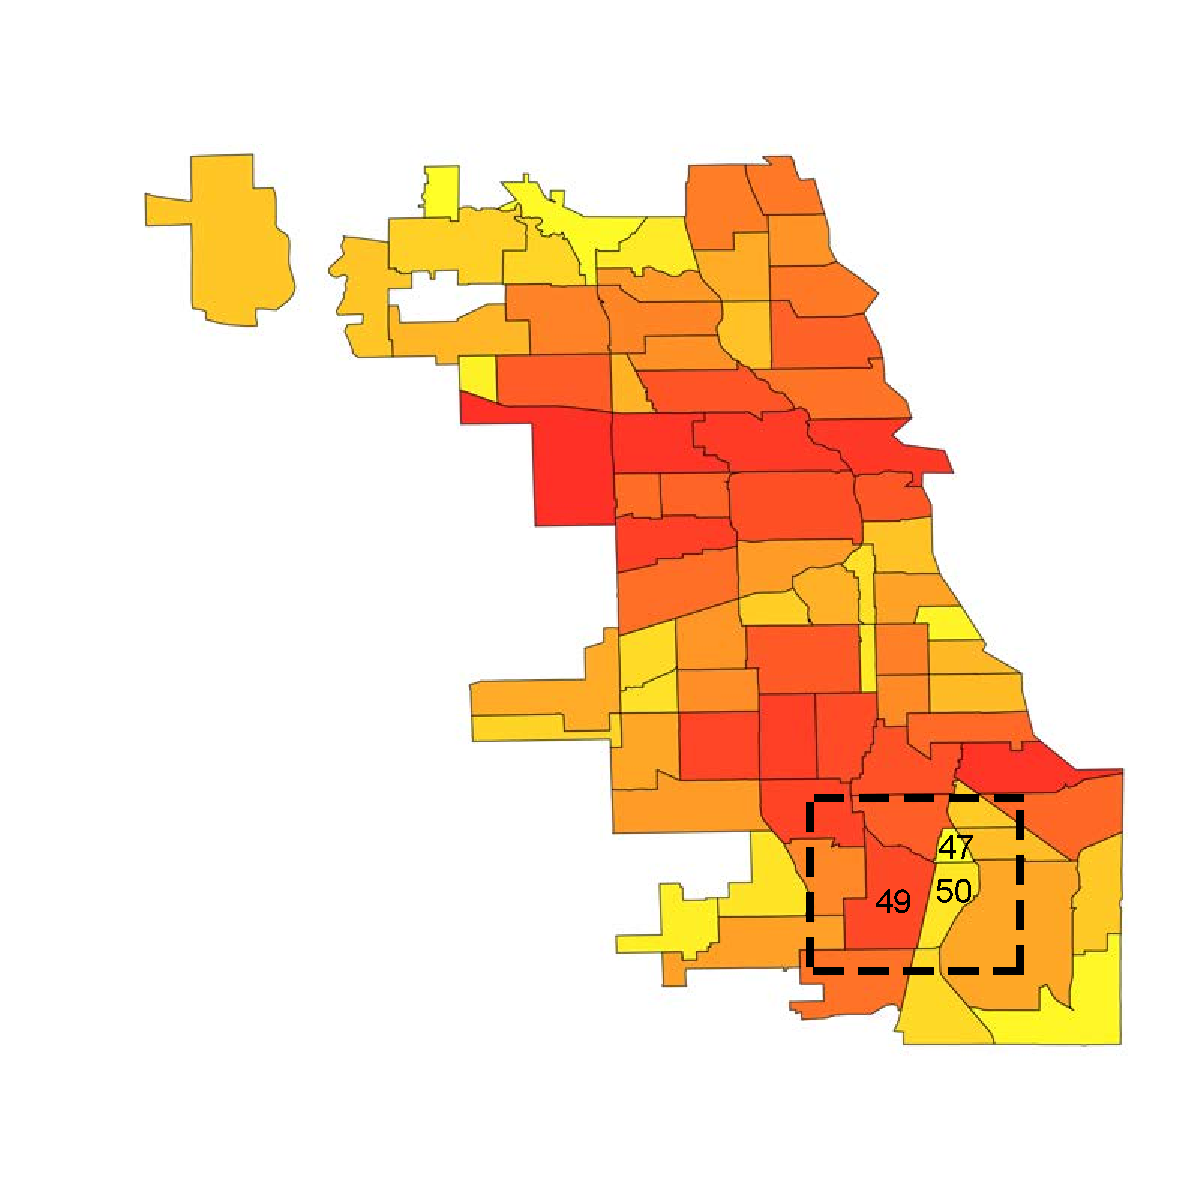
\includegraphics[width=0.3\linewidth]{fig/before-total-all-final.pdf}}
\subfigure[Crime Before]{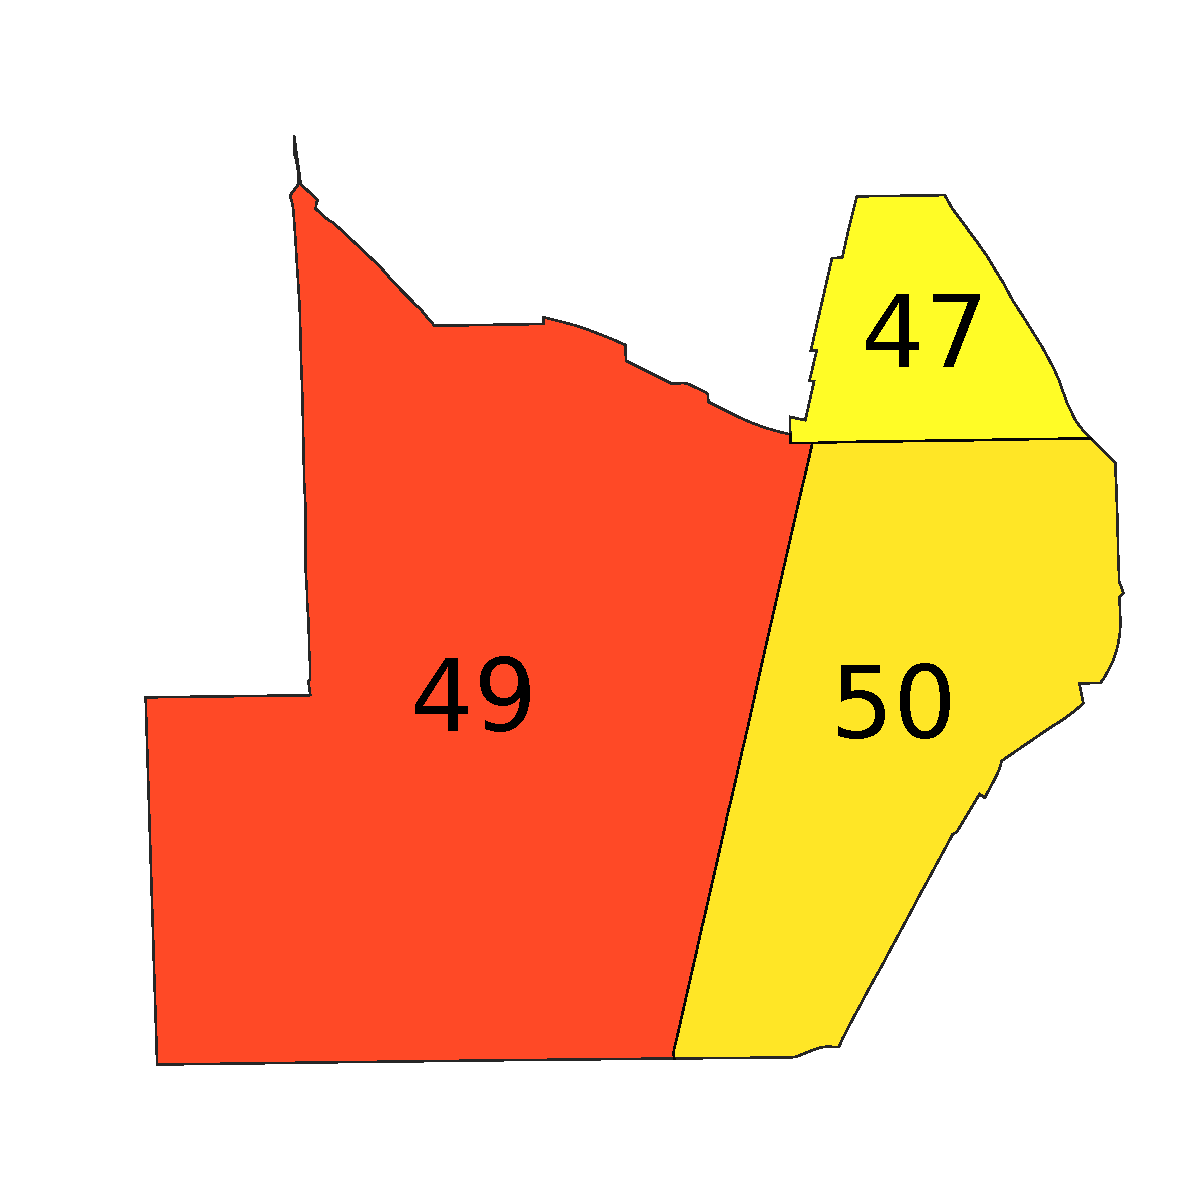
\includegraphics[width=0.28\linewidth]{fig/before-total.pdf}}
\subfigure[Poverty Before]{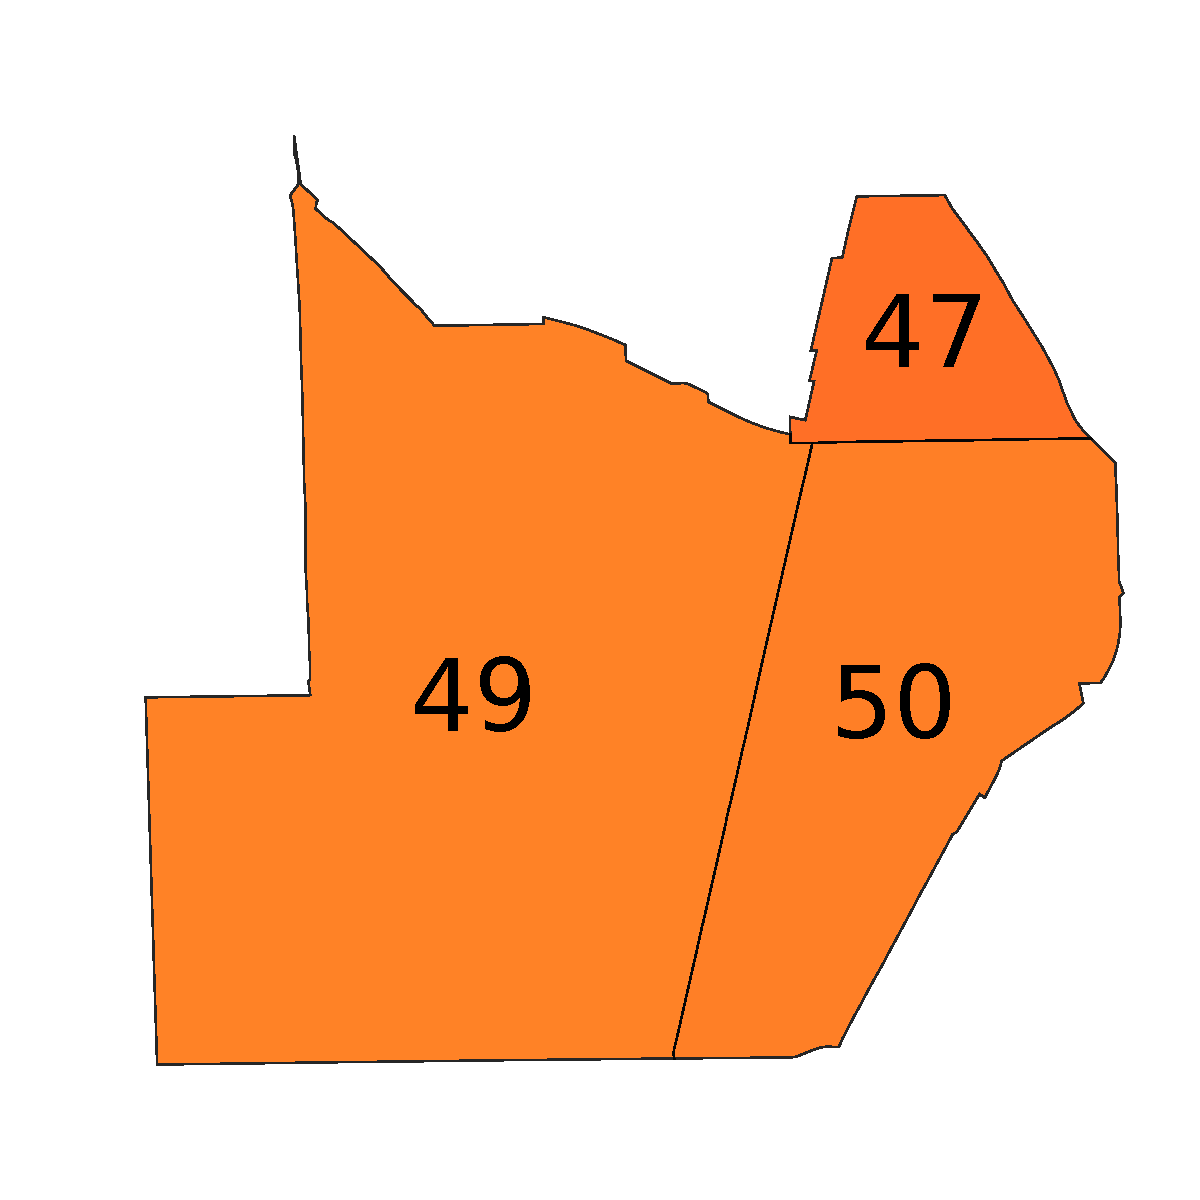
\includegraphics[width=0.28\linewidth]{fig/before-poverty_index.pdf}}
\subfigure[Crime After]{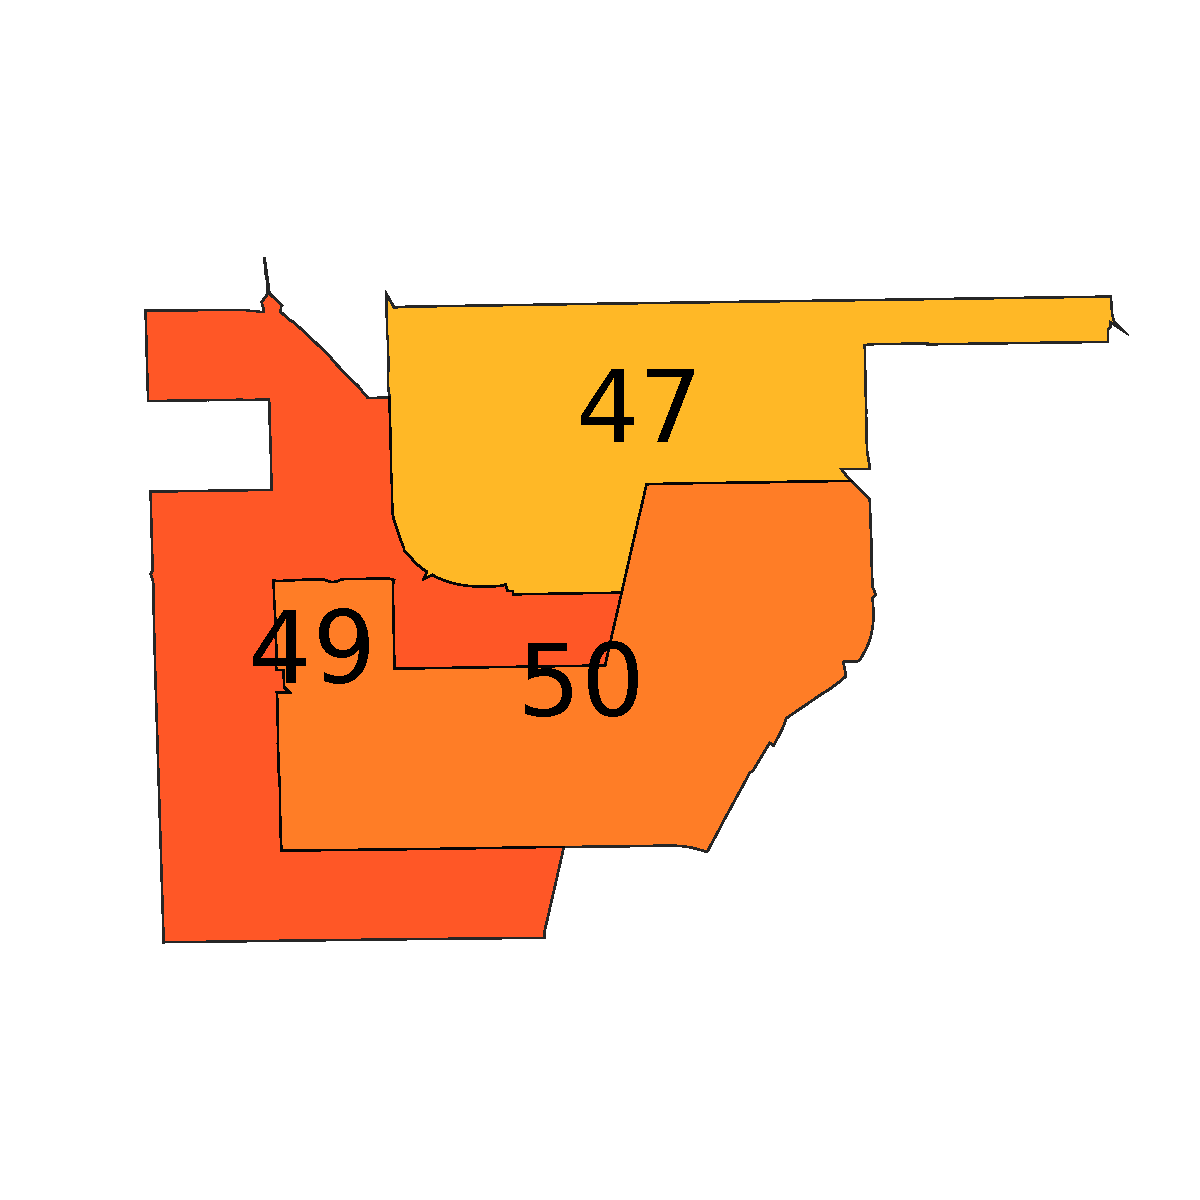
\includegraphics[width=0.32\linewidth]{fig/after-total.pdf}}
\subfigure[Poverty After]{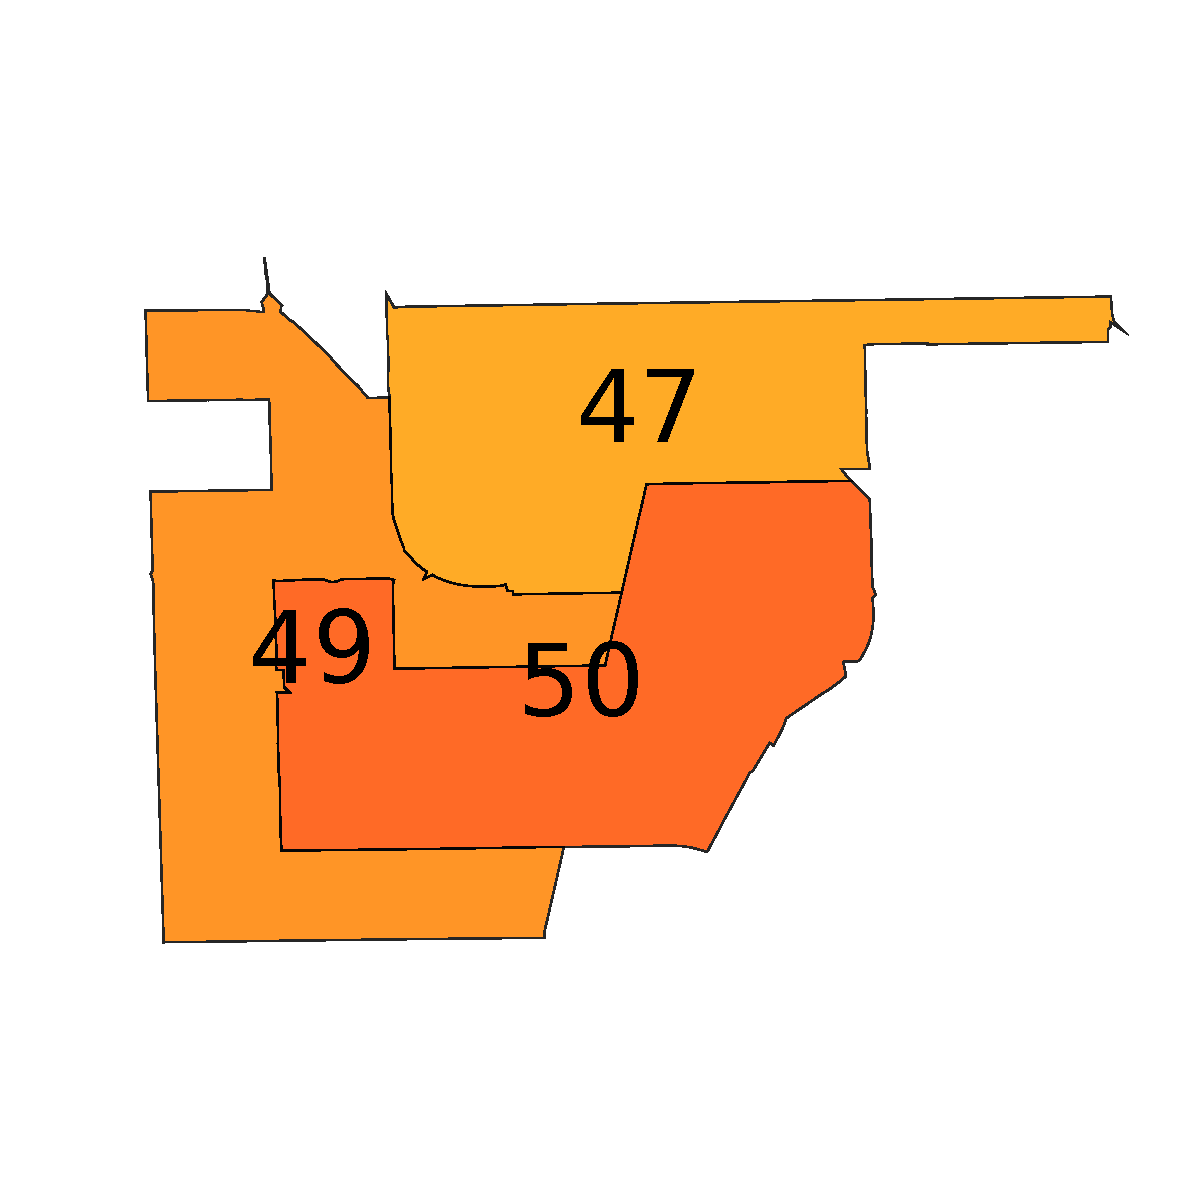
\includegraphics[width=0.32\linewidth]{fig/after-poverty_index.pdf}}
\caption{Crime prediction case near Community \#47. (a) Crime count distribution in Chicago under \texttt{Admin} partition. Dotted rectangle denotes the region of interest. (b) Crime count in region of interest under \texttt{Admin} partition. (c) Poverty index in region of interest under \texttt{Admin} partition. (d) Crime count in region of interest under \texttt{DQN} partition. (e) Poverty index in region of interest under \texttt{DQN} partition.}
\label{fig:crime-case}
\end{figure*}

\smallskip
\textbf{Crime prediction case study}. For crime study, we give the intuition why our partition gives lower prediction errors in the corresponding task. The case is shown in Figure~\ref{fig:crime-case}.

For the purpose of simplicity, we choose a single feature, that reasonably correlates with our variable of interest, namely crime count. The single feature we choose is the poverty index, which is calculated by the percentage of households in a given community whose combined income is less than or equal to \$30, 000. Figure~\ref{fig:crime-case}(a) shows a heat map of crime count by community, using the original administrative boundary. Warmer areas correspond to higher crime counts. We focus on communities \#47, \#49, and \#50, as marked by the dotted rectangle in Figure~\ref{fig:crime-case}(a). 


A zoom-in plot of the crime count by administrative boundary is shown in Figure~\ref{fig:crime-case}(b). Additionally, we construct a similar plot of the poverty index of these three communities, found in Figure~\ref{fig:crime-case}(c). It is clear that under  \texttt{Admin} partition, these communities are nearly identical in poverty index, while their crime counts differ dramatically. Next, we visualize the crime count and poverty index with  \texttt{DQN} partition in Figure~\ref{fig:crime-case}(d) and Figure~\ref{fig:crime-case}(e), respectively. We can see that these three regions of interest still exhibit similar poverty levels, but their crime counts are much closer to each other.


The observation above reveals the intuition of  \texttt{DQN} partition: it attempts to make the spatial distributions of $X$ and $Y$ similar. In other words, this is how  \texttt{DQN} partition reduces the prediction error.

We also note that community \#47 dramatically increased in size under  \texttt{DQN} partition. Community \#47 used to be the smallest community according to the Chicago's administrative boundary partition, with a population of less than 3,000 people. The variance penalty in our objective function (Equation~\ref{eq:objective}) causes our proposed method to favor regions that are similar in terms of population. It is likely that this community is expanded to yield better correlation between poverty and crime, as well as balance out the population distribution over communities.




